\chapter{Durchführung}

\section{Fluss des Prozesses}

Für die Durchführung dieses Prozess wurden die Tabellen \texttt{co6\_config\_variables} des Schemas \texttt{copra}; \texttt{loinc} und \texttt{loinc\_german\_translation} aus dem Schema \texttt{loinc}. Von diesen Tabellen \texttt{co6\_config\_variables} und \texttt{loinc\_german\_translation} wurden die notwendigen Spalten ausgewählt und für die Zuordnungen aufbereitet. Das Ergebnis dieser Aufbereitung wurden in \ac{csv}-Dateien exportiert und die ersten Zuordnungen wurde durchgeführt. En neues Schema wurde erstellt für die Speicherung der Zuordnungen. In diesem neuen Schema wurden die besten Zuordnungen ausgewählt und weitere Suchen mit Hilfe von \ac{regex} wurden durchgeführt. Dieser letzte Schritt war notwendig, denn nicht alle \ac{loinc}-Terminologien sind auf Deutsch übersetzt.

\begin{figure}[ht]
	\centering
	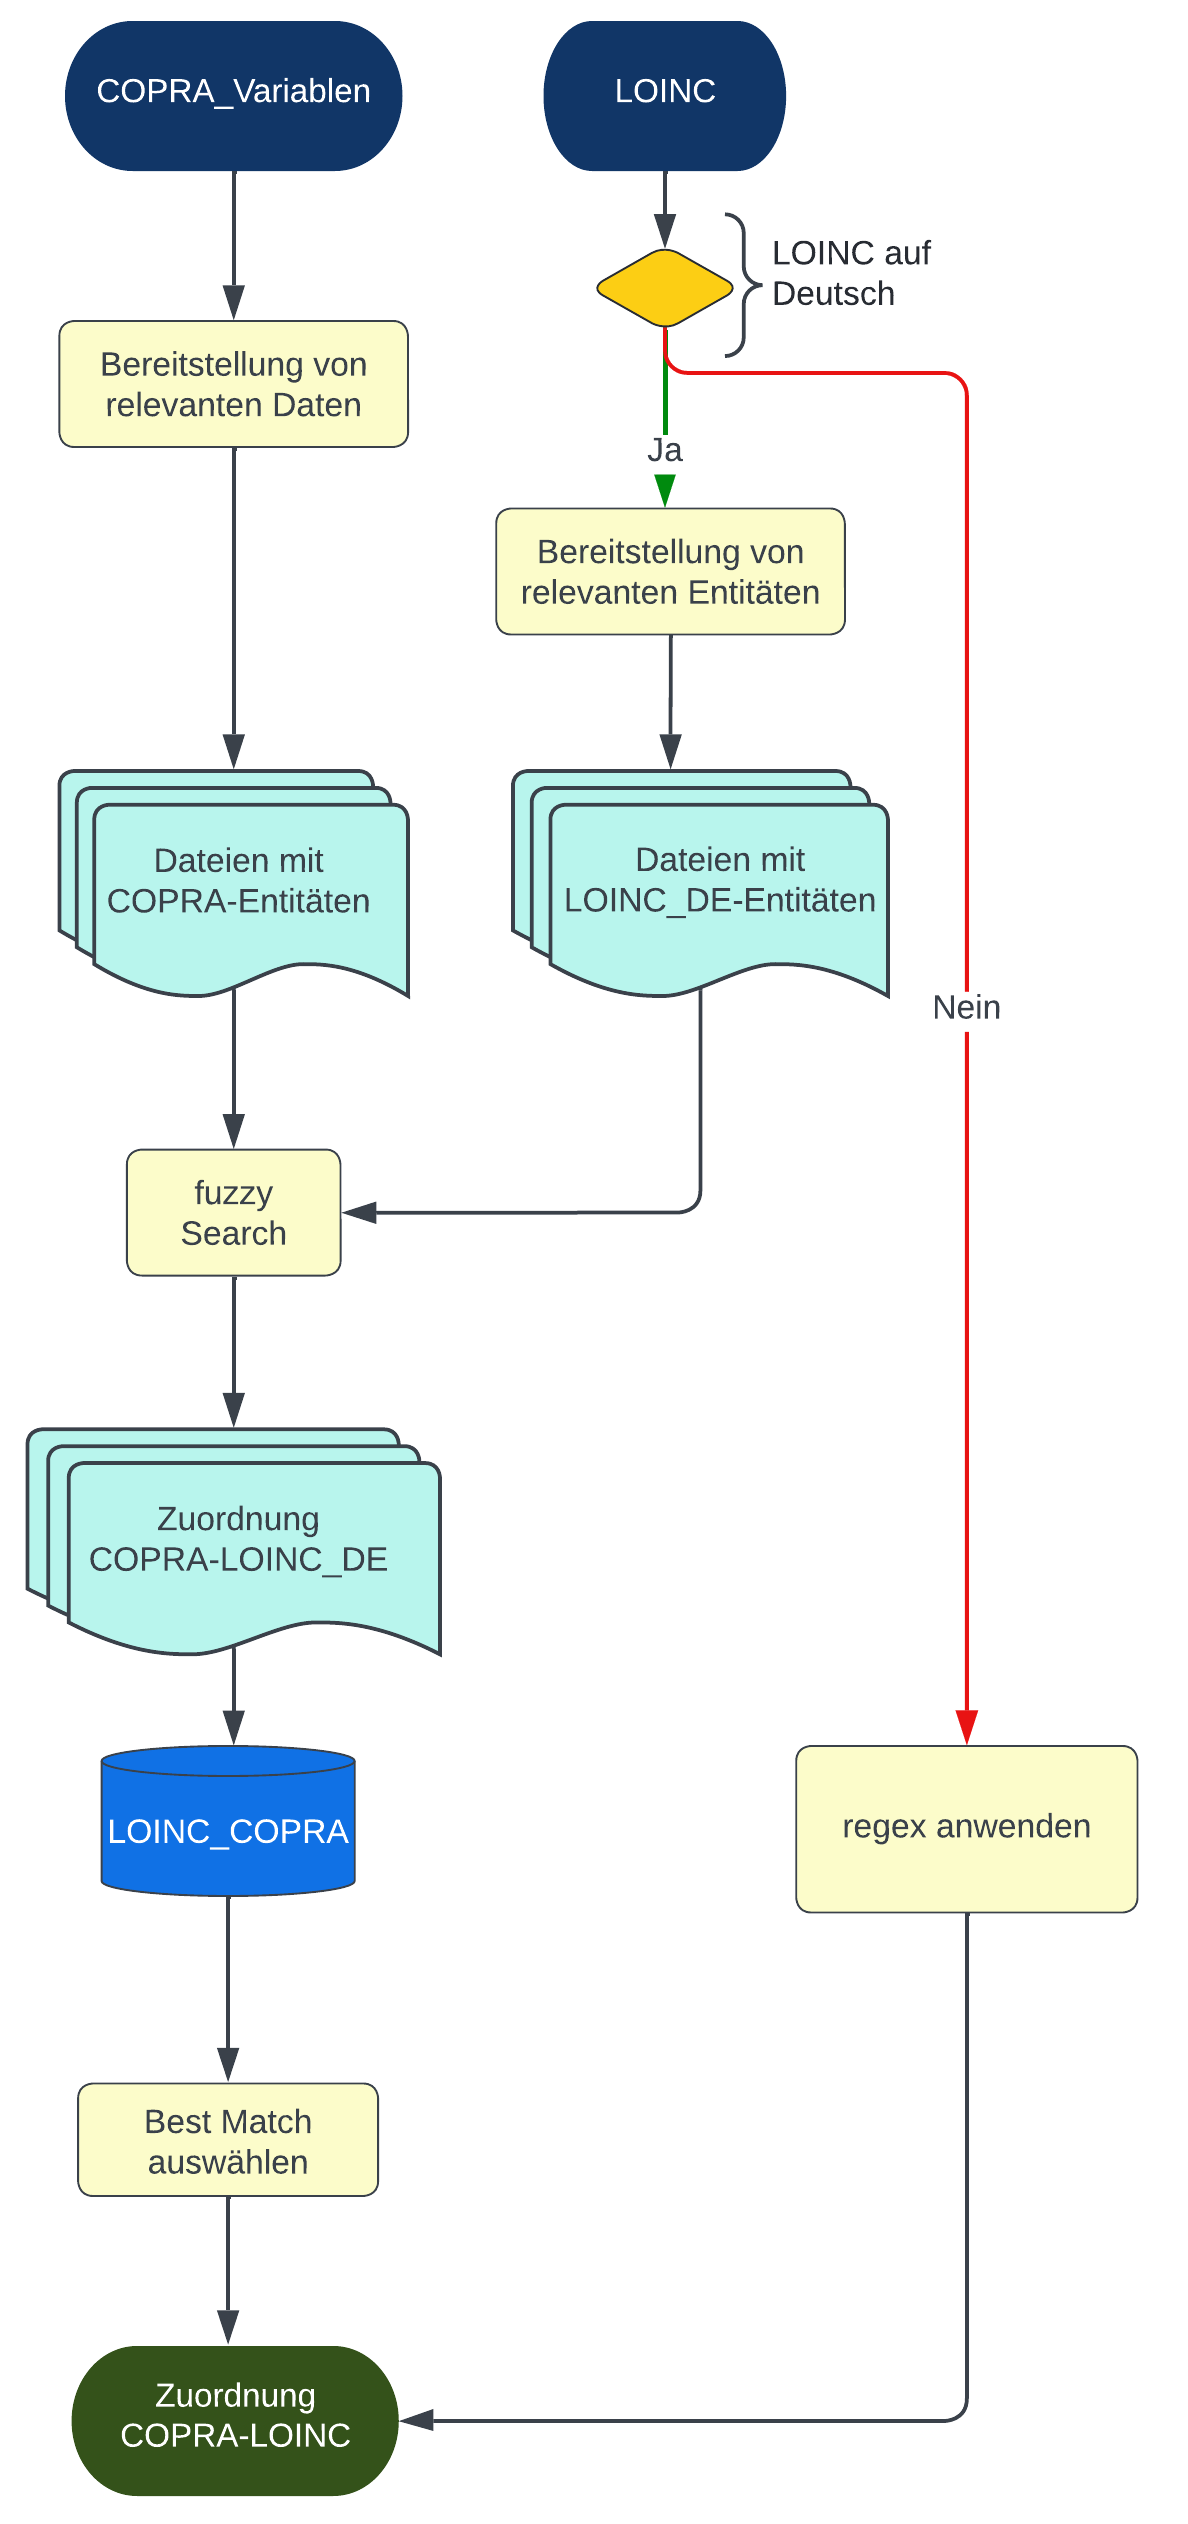
\includegraphics[height=10cm]{figures/copra_loinc}
	\caption[Flussdiagramm des Prozesses]{Flussdiagramm des Prozesses.}
	\label{fig:copraloinc}
\end{figure}